% chktex-file 3 chktex-file 9 chktex-file 13 chktex-file 17 chktex-file 18 chktex-file 36

\section{Ajustes y Pruebas de Ajuste para modelos ARMA}

\subsection*{9.3 Escogencia de Orden}

Las 3 funciones que califican la verosimilitud de un modelo $\ARMA$ con parámetros $(\bm{\beta},\sigma^2) = (\bm{\phi},\bm{\theta},\sigma^2)$ son

\[ \mbox{AIC}(\bm{\beta}) := -2 \ln L(\bm{\beta}, S(\bm\beta)/n) + 2(p+q+1) \]
\[ \mbox{AICC}(\bm{\beta}) := -2 \ln L(\bm{\beta}, S(\bm\beta)/n) + \frac{2(p+q+1)n}{(n-p-q-2)} \]
\[ \everymath{\displaystyle}
\arraycolsep=1.8pt\def\arraystretch{2}
\begin{array}{rcl}
    \mbox{BIC}(\bm{\beta}) & := & (n-p-q) \ln\left[ \frac{S(\bm\beta)}{n-p-q} \right] + n(1+\ln(\sqrt{2\pi}))\\
    & & + (p+q) \ln\left[ \frac{\sum_{t = 1}^n X_t^2 - S(\bm\beta)}{p+q} \right],
\end{array} \]

Para estimar $\wh{p},\wh{q}$ óptimos, calculamos el modelo de máxima verosimilitud $\tilde{\bm\beta}$ como en (8.7) para diferentes valores de $p,q$ y evaluamos en alguna de estas 3 funciones hasta encontrar el que la minimiza. De acuerdo a la discusión de 9.3 las funciones tienen pros y contras al ser usadas como criterios:
\begin{itemize}
    \item[(1)] AIC y AICC son estimadores de un estadístico llamado "Kullback-Leibler index" al cual al ser minimizado se maximiza la función de verosimilitud.
    \item[(2)] AIC y AICC son equivalentemente asintóticos. AIC tiende a sobreestimar $p$, pero, para modelos de gran orden es mejor que AICC.
    \item[(3)] Entre los 3, el único que produce estadísticos consistentes $\wh{p} \to p$, $\wh{q}\to q$ es BIC. Sin embargo, a diferencia de AIC y AICC, el cálculo de BIC no es asintóticamente eficiente para modelos autorregresivos.
\end{itemize}

\subsection*{9.4 Test de Residuales}

Para un modelo $\ARMA$ $X_t$ con parámetro $\bm\beta = (\bm\phi,\bm\theta)$ se observan datos $X_1, \ldots, X_n$. A partir de estas observaciones se calculan predicciones en base a un parámetro $\wh{\bm\beta} = (\wh{\bm\phi},\wh{\bm\theta})$. Para las predicciones en base a los parámetros reales $\wh{X}_{n+1} = \wh{X}_{n+1}(\bm\phi,\bm\theta) = P_n X_{n+1}$, los residuos "reales":
\[ W_n(\bm{\phi},\bm{\theta}) = (X_{n}-\wh{X}_{n})/\sqrt{r_{n-1}(\bm{\phi},\bm{\theta})} \]
debería comportarse, de acuerdo con la discusión del capitulo 8, como ruido blanco. De la misma forma, para los residuos de los parámetros estimados
\[  \wh{W}_n(\wh{\bm{\phi}},\wh{\bm{\theta}}) = (X_{n}-\wh{X}_{n}(\wh{\bm{\phi}},\wh{\bm{\theta}}))/\sqrt{r_{n-1}(\wh{\bm{\phi}},\wh{\bm{\theta}})}, \]
debería suceder lo mismo. En particular, $\E[( W_n(\bm{\phi},\bm{\theta}) - Z_n)^2] \to 0$ cuando $n \to \infty$ y por lo tanto,
\begin{itemize}
    \item[(1)] Si $Z_t \sim \WN(0,\sigma^2)$, entonces el proceso $\wh{W}_n$ debería tener covarianzas pequeñas.
    \item[(2)] Si $Z_t \sim \mbox{IID}(0,\sigma^2)$, entonces el proceso $\wh{W}_n$ es independiente.
    \item[(3)] Si $Z_t \sim \mathcal{N}(0,\sigma^2)$, entonces la distribución del proceso $\wh{W}_n$ debería parecerse a una gaussiana.
\end{itemize}

La función de autocovarianzas muestrales de $\wh{W}_t$ se define de la siguiente forma
\[ \wh{\rho}_W(h) = \frac{\sum_{t = 1}^{n-h}(\wh{W}_{t} - \ol{W})(\wh{W}_{t+h}- \ol{W})}{\sum_{t = 1}^n (\wh{W}_t- \ol{W})^2}, \]
en donde $\ol{W} = n^{-1}\sum_{t = 1}^n \wh{W}_{t}$.

\begin{figure}[H]
    \centering
    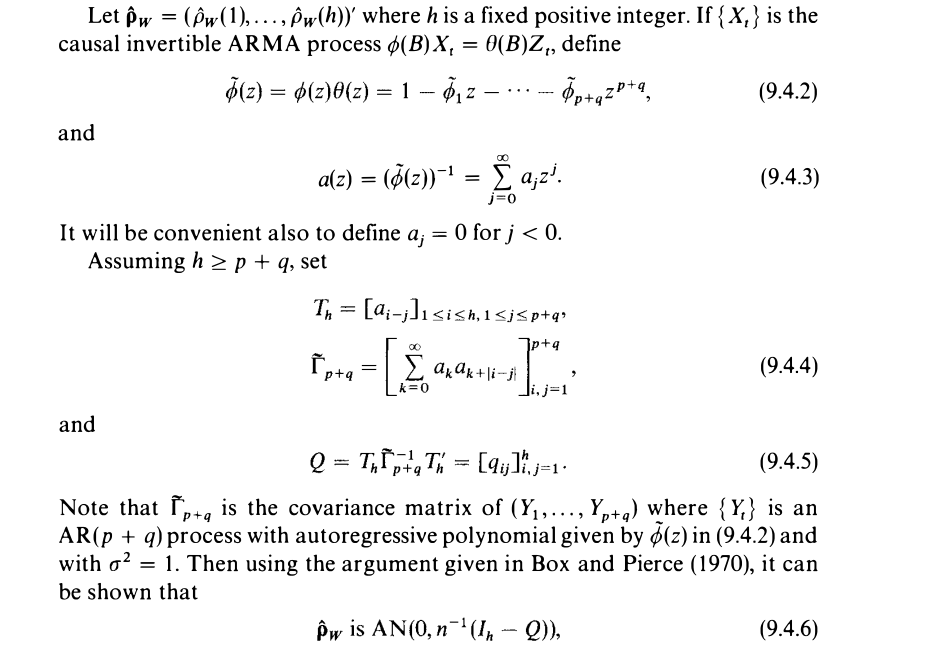
\includegraphics[width=1\textwidth]{../pictures/image6.png}
\end{figure}

\begin{figure}[H]
    \centering
    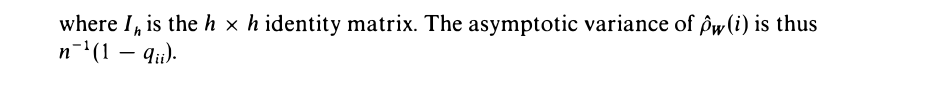
\includegraphics[width=1\textwidth]{../pictures/image7.png}
\end{figure}

\begin{figure}[H]
    \centering
    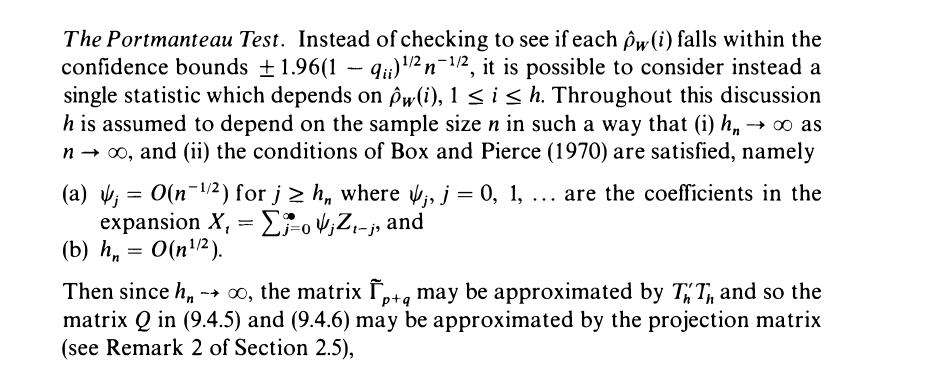
\includegraphics[width=1\textwidth]{../pictures/image8.png}
\end{figure}

\begin{figure}[H]
    \centering
    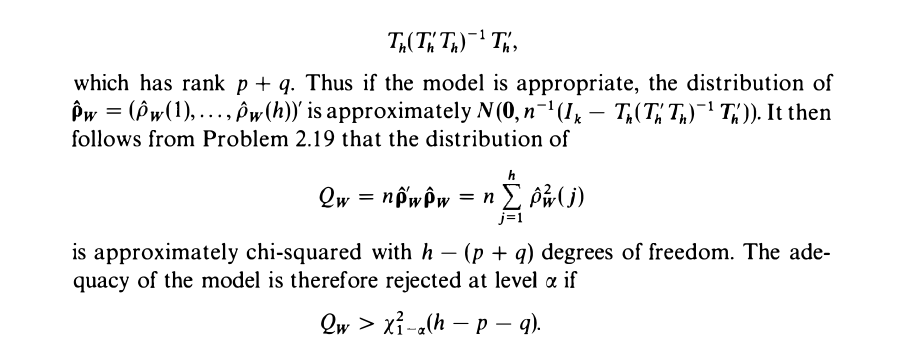
\includegraphics[width=1\textwidth]{../pictures/image9.png}
\end{figure}

\subsection*{Kullback-Leibler Index}

\begin{figure}[H]
    \centering
    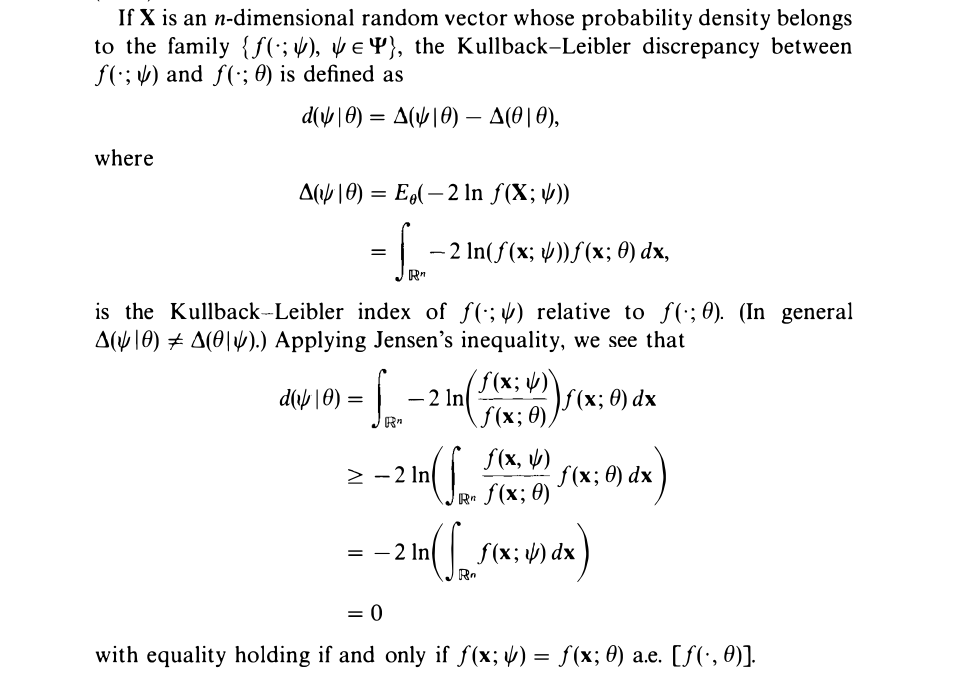
\includegraphics[width=1\textwidth]{../pictures/image10.png}
\end{figure}

\begin{figure}[H]
    \centering
    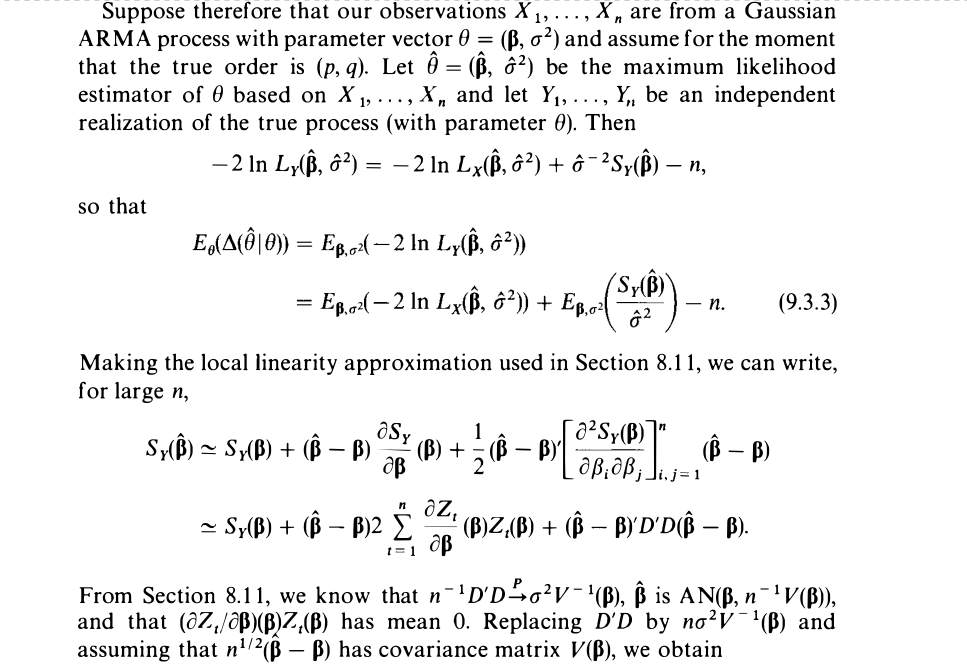
\includegraphics[width=1\textwidth]{../pictures/image11.png}
\end{figure}

\begin{figure}[H]
    \centering
    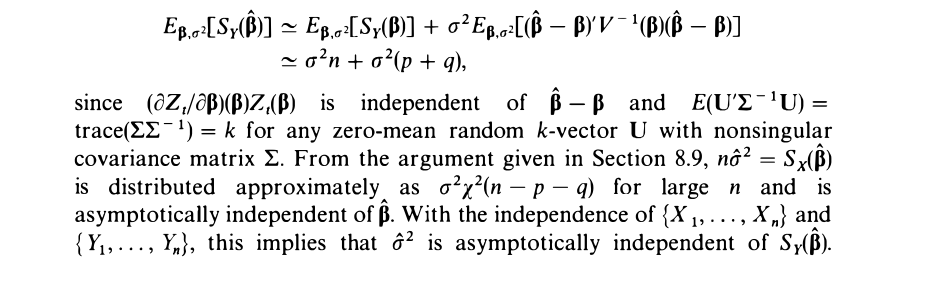
\includegraphics[width=1\textwidth]{../pictures/image12.png}
\end{figure}

\begin{figure}[H]
    \centering
    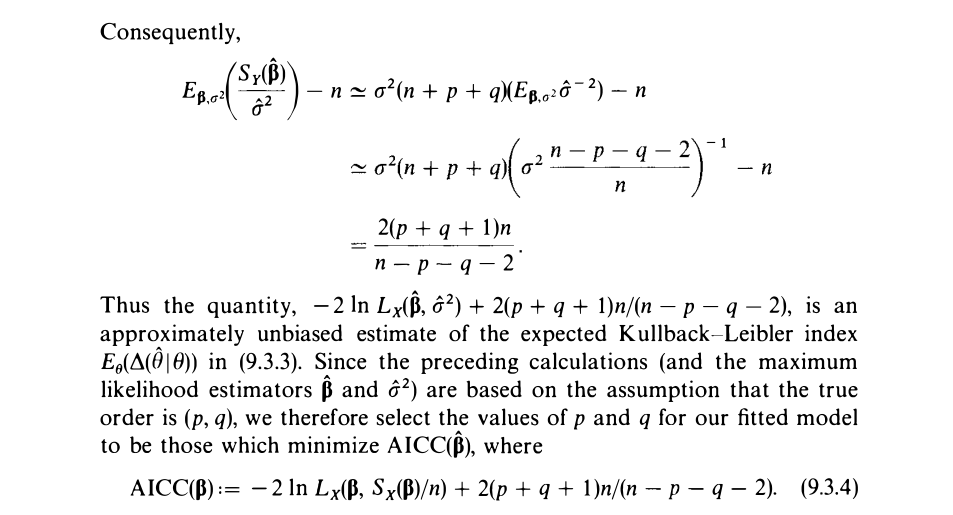
\includegraphics[width=1\textwidth]{../pictures/image13.png}
\end{figure}